\textit{The process of developing for Android, how an app is installed and how it is being run is explained in this chapter. Additionally, common optimization techniques are described so that we can reason about the results. Lastly, some basic knowledge of the Discrete Fourier Transform is required when discussing differences in FFT implementations. }

\section{Android SDK}
To allow developers to build Android apps, Google developed a Software Development Kit (\gls{sdk}) to facilitate the process of writing Android applications. The Android \gls{sdk} software stack is described in Figure~\ref{fig:sdk}. The Linux kernel is at the base of the stack, handling the core functionality of the device. Detecting hardware interaction, process scheduling and memory allocation are examples of services provided by the kernel. The Hardware Abstraction Layer (\gls{hal}) is an abstraction layer above the device drivers. This allows the developer to interact with hardware independent on the type of device \cite{android:hal}.

The native libraries are low level libraries, written in C or C++, that handle functionality such as the Secure Sockets Layer (\gls{ssl}) and Open GL \cite{komatineni2012pro}. Android Runtime (\gls{art}) features Ahead-Of-Time (\gls{aot}) compilation and Just-In-Time (\gls{jit}) compilation, garbage collection and debugging support \cite{android:sdk:stack}. This is where the Java code is being run and because of the debugging and garbage collection support, it is also beneficial for the developer to write applications against this layer.

The Java \gls{api} Framework is the Java library you use when controlling the Android UI. It is the reusable code for managing activities, implementing data structures and designing the application. The System Application layer represents the functionality that allows a third-party app to communicate with other apps. Example of usable applications are email, calendar and contacts \cite{android:sdk:stack}.

All applications for Android are packaged in so called Android Packages (\gls{apk}). These APKs are zipped archives that contain all the necessary resources required to run the app. Such resources are the AndroidManifest.xml file, Dalvik executables (.dex files), native libraries and other files the application depends on.

\ifrelease
\begin{figure}
    \centering

    \begin{tikzpicture}[node distance=3pt,outer sep=0pt,
            blueb/.style={
                draw=white,
                fill=mybluei,
                rounded corners,
                text width=2.5cm,
                font={\sffamily\bfseries\color{white}},
                align=center,
                text height=12pt,
            text depth=9pt},
            greenb/.style={blueb,fill=mygreen},
            darkgreenb/.style={blueb,fill=mydarkgreen},
            redb/.style={blueb,fill=myred},
            greyb/.style={blueb,fill=mygrey},
            yellowb/.style={blueb,fill=myyellow},
        ]

        \node[label=center:{\sffamily\bfseries\color{white}System Applications},darkgreenb,minimum width=15.9cm] (SysApps) {};

        \node[label=center:{\sffamily\bfseries\color{white}Java API Framework},greenb,minimum width=15.9cm,below=of SysApps] (JAPI) {};

        \node[label=center:{\sffamily\bfseries\color{white}Native Libraries},greyb,below=of JAPI,minimum width=13cm,xshift=-1.45cm] (Nat) {};
        \node[label=center:{\sffamily\bfseries\color{white}ART},yellowb,right=of Nat] (Art) {};

        \widernode{Nat}{Art}{Hardware Abstraction Layer (HAL)}{Hal}

        \widernode[redb]{Hal}{Hal}{Linux Kernel}{RCP}
        \begin{pgfonlayer}{background}
            \draw[blueb,draw=black,fill=mybluei!40] 
                ([xshift=-\myframesep,yshift=3\myframesep]current bounding box.north west) 
                rectangle 
                ([xshift=\myframesep,yshift=-\myframesep]current bounding box.south east);
        \end{pgfonlayer}
        \node[font=\sffamily\itshape\color{black},above=of SysApps] {Android SDK Software Stack};
    \end{tikzpicture}
    \caption[Android SDK Software Stack]{Android SDK Software Stack \cite{android:sdk:stack}}
    \label{fig:sdk}
\end{figure}
\fi


\section{Dalvik Virtual Machine}
% Why is Dalvik Virtual Machine used?
Compiled Java code is executed on a virtual machine called the Java Virtual Machine (\gls{jvm}). The reason for this is to allow portable compiled code. This way, every device, independent on architecture, with a \gls{jvm} installed will be able to run the same code. The Android operating system is designed to be installed on many different devices \cite{android:os:devices}. Compiling to machine code for the targeted devices could become impractical because a program must be compiled against all possible platforms it should work on. For this reason, Java bytecode is a sensible choice when wanting to distribute compiled applications.

The Dalvik Virtual Machine (\gls{dvm}) is the VM initially used on Android. One difference between \gls{dvm} and \gls{jvm} is that the \gls{dvm} uses a register-based architecture while the \gls{jvm} uses a stack-based architecture. The most common virtual machine architecture is the stack-based \cite[p.~158]{craig2010virtual}. A stack-based architecture evaluates each expression directly on the stack and always has the last evaluated value on top of the stack. Thus, only a stack pointer is needed to find the next instruction on the stack.

Contrary to this behaviour, a register-based virtual machine works more like a CPU. It uses a set of registers where it will place operands by fetching them from memory. One advantage of using a register-based architecture is that fetching data between registers is faster than fetching or storing data onto the hardware stack. The biggest disadvantage of using register-based architecture is that the compilers must be more complex than for stack-based architecture. This is because the code generators must take register management into consideration~\cite[p.~159-160]{craig2010virtual}.

The \gls{dvm} is a virtual machine optimized for devices where resources are limited \cite{android:dalvik:internals}. The main focus of the \gls{dvm} is to lower memory consumption and lower the number of instructions needed to fulfil a task. Using register-based architecture, it is possible to execute more virtual machine instructions compared to a stack-based architecture \cite{shi2008virtual}. 

% http://www.android-app-developer.co.uk/android-app-development-docs/android-jit-compiler-androids-dalvik-vm.pdf
% https://developer.android.com/about/versions/nougat/android-7.0.html

Dalvik executables, or \gls{dex} files, are the files where Dalvik bytecode is stored. They are created by converting a Java .class file to the \gls{dex} format. They are of a different structure than the Java .class files. One difference is the header types that describes the data. Another difference is the string constant fields that are present in the \gls{dex}-file. % FIND REFERENCE FROM GOOGLE IO ABOUT DALVIK??

\section{Android Runtime}
Android Runtime is the new default runtime for Android as of version 5.0 \cite{android:dalvik}. The big improvement over Dalvik is the fact that applications are compiled to binary when they are installed on the device, rather than during runtime of the app. This results in faster start-up \cite{li2016advanced} and lets the compiler use more heavy optimization that is not otherwise possible during runtime. However, if the whole application is compiled ahead of time it is no longer possible to do any runtime optimizations. An example of a runtime optimization is to inline methods or functions that are called frequently.

When an app is installed on the device, a program called \textbf{dex2oat} converts a \gls{dex}-file to an executable file called an oat-file \cite{android:art:dalvik}. This oat-file is in the Executable and Linkable Format (ELF) and can be seen as a wrapper of multiple \gls{dex}-files \cite{Dresel2016}. An improvement made in Android Runtime is the optimized garbage collector. Changes include a decrease from two to one GC pause, reduced memory fragmentation (reduces calls to \texttt{GC\_FOR\_ALLOC}) and parallelization techniques to lower the time it takes to collect garbage~\cite{android:art:dalvik}. There are two common garbage collects plans, Sticky Concurrent Mark Sweep (Sticky CMS) and Partial Concurrent Mark Sweep (Partial CMS). Sticky CMS does not move data and does only reclaim data that has been allocated since the last garbage collect \cite{android:art:gc}. Partial CMS frees from the active heap of the process \cite[p.~122]{sillars2015high}.

\section{Native Development Kit}
Native Development Kit (\gls{ndk}) is a set of tools to help write native apps for Android. It contains the necessary libraries, compilers, build tools and debugger for developing low level libraries. Google recommends using the \gls{ndk} for two reasons: run computationally intensive tasks and usage of already written libraries \cite{android:ndk:guides}. Because Java is the supported language on Android, due to security and stability, native development is not recommended to use when building full apps, with an exception of when developing games.

Historically, native libraries have been built using Make. Make is a tool used to coordinate compilation of source files. Android makefiles, \texttt{Android.mk} and \texttt{Application.mk}, are used to set compiler flags, choose which architectures that a project should be compiled for, location of source files and more. With Android Studio 2.2 \gls{cmake} was introduced as the default build tool \cite{android:studio:cmake}. CMake is a more advanced tool for generating and running build scripts.

At each compilation, the architectures the source files will be built against must be specified. The source file(s) generated will be placed in a folder structure (shown below) where the compiled source file is located in a folder that determines the architecture. Each architecture-folder is located in a folder called \texttt{lib}. This folder will be placed at the root of the \gls{apk}.

\begin{verbatim}
lib/
|--armeabi-v7a/
|  |--lib[libname].so
|--x86/
   |--lib[libname].so
\end{verbatim}

\subsection{Java Native Interface}
% GOOD => https://www.fer.unizg.hr/_download/repository/jni.pdf <=
To be able to call native libraries from Java code, a framework named Java Native Interface (\gls{jni}) is used. Using this interface, C/C++ functions are mapped as methods and primitive data types are converted between Java and C/C++. For this to work, special syntax is needed for \gls{jni} to recognize which method in which class a native function should correspond to.

To mark a function as native in Java, a special keyword called \texttt{native} is used to define a method. The library which implements this method must also be included in the same class. By using the \texttt{System.loadLibrary("mylib")} call, we can specify the name of the static library that should be loaded. Inside the native library we must follow a function naming convention to map a method to a function. The rules are that you must start the function name with \texttt{Java} followed by the package, class and method name. Figure~\ref{fig:native} demonstrates how to map a method to a native function.

\ifrelease
\begin{figure}[H]
\begin{center}
    \texttt{private native int myFun();}\\
    $\Updownarrow$
    \begin{verbatim}
      JNIEXPORT jint JNICALL
      Java_com_example_MainActivity_myFun (JNIEnv *env, jobject thisObj)
    \end{verbatim}
\end{center}
\caption{Native method declaration to implementation.}
\label{fig:native}
\end{figure}
\fi

The \gls{jni} also provides a library for C and C++ for handling the special \gls{jni} data types. They can be used to determine the size of a Java array, get position of elements of an array and handling Java objects. In C and C++ you are given a pointer to a list of \gls{jni} functions (\texttt{JNIEnv*}). With this pointer, you can communicate with the JVM \cite[p.~22]{liang1999java}. You typically use the \gls{jni} functions to fetch data handled by the JVM, call methods and create objects.

The second parameter to a \gls{jni} function is of the \texttt{jobject} type. This is the current Java object that has called this specific \gls{jni} function. It can be seen as an equivalent to the \texttt{this} keyword in Java and C++ \cite[p.~23]{liang1999java}. There is a function-pair available in the \texttt{JNIEnv} pointer called \texttt{GetDoubleArrayElements()} and \texttt{ReleaseDoubleArrayElements()}. There are also functions for other primitive types such as \texttt{GetIntArrayElements()}, \texttt{GetShortAr\-rayElements()} and others. \texttt{GetDoubleArrayElements()} is used to convert a Java array to a native memory buffer \cite[p.~159]{liang1999java}. This call also tries to \enquote{pin} the elements of the array.

\emph{Pinning} allows \gls{jni} to provide the reference to an array directly instead of allocating new memory and copying the whole array. This is used to make the call more efficient although it is not always possible. Some implementations of the virtual machine does not allow this because it requires that the behaviour of the garbage collector must be changed to support this \cite[p.~158]{liang1999java}. There are two other functions, \texttt{GetPrimitiveArrayCritical()} and \texttt{ReleasePrimitiveArrayCritical()}, that can be used to avoid garbage collection in native code. Between these function calls, the native code should not run forever, no calls to any of the \gls{jni} functions are allowed and it is prohibited to block a thread that depends on a VM thread to continue.

\subsection{LLVM and Clang}
\gls{llvm} (Low Level Virtual Machine) is a suite that contains a set of compiler optimizers and backends. It is used as a foundation for compiler frontends and supports many architectures. An example of a frontend tool that uses \gls{llvm} is \gls{clang}. Clang is used compile C, C++ and Objective-C source code \cite{clang:comp}.

Clang is as of March 2016 (\gls{ndk} version 11) \cite{android:ndk:revision}, the only supported compiler in the \gls{ndk}. Google has chosen to focus on supporting the Clang compiler instead of the GNU GCC compiler. This means that there is a bigger chance that a specific architecture used on an Android device is supported by the \gls{ndk}. This also allows Google to focus on developing optimizations for these architectures with only one supported compiler.

\section{Code Optimization}

There are many ways your compiler can optimize your code during compilation. This chapter will first present some general optimization measures taken by the optimizer and will then describe some language specific methods for optimization.

\subsubsection{Loop unrolling}
Loop unrolling is a technique used to optimize loops. By explicitly having multiple iterations in the body of the loop, it is possible to lower the amount of jump instructions in the produced code. Figure~\ref{fig:c:unroll} demonstrates how unrolling works by decreasing the number of iterations while adding lines in the loop body. The loop unroll executes two iterations of the first code per iteration. It is therefore necessary to update the \texttt{i} variable accordingly. Figure~\ref{fig:assembly:unroll} describes how the change could be represented in assembly language.

\ifrelease
\begin{figure}
    \centering
    \begin{subfigure}{.5\textwidth}
        \centering
        \begin{verbatim}
    for (int i = 0; i < 6; ++i) {
        a[i] = a[i] + b[i];
    }

        \end{verbatim}
        \caption{Normal}
        \label{fig:c:unroll:normal}
    \end{subfigure}%
    \begin{subfigure}{.5\textwidth}
        \centering
        \begin{verbatim}
    for (int i = 0; i < 6; i+=2) {
        a[i] = a[i] + b[i];
        a[i+1] = a[i+1] + b[i+1];
    }
        \end{verbatim}
        \caption{One unroll}
        \label{fig:c:unroll:unroll}
    \end{subfigure}
    \caption{Loop unrolling in C}
    \label{fig:c:unroll}
\end{figure}
\fi

The gain in using loop unrolling is that you \enquote{save} the same amount of jump instructions as the amount of \enquote{hard coded} iterations you add. In theory, it is also possible to optimize even more by changing the offset of \texttt{LOAD WORD} instructions as shown in Figure~\ref{fig:assembly:optimized}. Then you would not need to update the iterator as often.

% https://www.cs.umd.edu/class/fall2001/cmsc411/proj01/proja/why.html
\ifrelease
\begin{figure}
    \centering
    \begin{adjustbox}{minipage=\linewidth,scale=0.8}
        \begin{verbatim}
                $s1 - a[] address | $s4 - value of a[x]
                $s2 - b[] address | $s5 - value of b[x]
                $s3 - i           | $s6 - value 6
        \end{verbatim}
        \begin{subfigure}{.55\textwidth}
            \centering
            \begin{lstlisting}[
                    language={[mips]Assembler},
                    basicstyle=\footnotesize,
                    numbers=left,
                    firstnumber=1,
                    numberfirstline=true
                ]
loop: lw $s4, 0($s1) # Load a[i]
      lw $s5, 0($s2) # Load b[i]
      add $s4, $s4, $s5 # a[i] + b[i]
      sw $s4, 0($s1)
      addi $s1, $s1, 4 # next element
      addi $s2, $s2, 4 # next element
      addi $s3, $s3, 1 # i++
      bge $s3, $s6, loop
                \end{lstlisting}
            \caption{Normal}
            \label{fig:unroll:sub1}
        \end{subfigure}%
        \begin{subfigure}{.3\textwidth}
            \centering
            \begin{lstlisting}[
                    language={[mips]Assembler},
                    basicstyle=\footnotesize,
                    numbers=left,
                    firstnumber=1,
                    numberfirstline=true
                ]
loop: lw $s4, 0($s1)
      lw $s5, 0($s2)
      add $s4, $s4, $s5
      sw $s4, 0($s1)
      addi $s1, $s1, 4
      addi $s2, $s2, 4
      addi $s3, $s3, 1
      lw $s4, 0($s1)
      lw $s5, 0($s2)
      add $s4, $s4, $s5
      sw $s4, 0($s1)
      addi $s1, $s1, 4
      addi $s2, $s2, 4
      addi $s3, $s3, 1
      bge $s3, $s6, loop
                \end{lstlisting}
            \caption{One unroll}
            \label{fig:unroll:sub2}
        \end{subfigure}
    \end{adjustbox}
    \caption{Loop unrolling in assembly}
    \label{fig:assembly:unroll}
\end{figure}
\fi


\subsubsection{Inlining}
Inlining allows the compiler to swap all the calls to an inline function with the content of the function. This removes the need to do all the preparations for a function call such as saving values in registers and preparing parameters and return values. This comes at a cost of a larger program if there are many calls to this function in the code and if the function is large. It is very useful to use inline functions in loops that are run many times. This is an optimization that can be requested in C and C++ by using the \texttt{inline} keyword and can also be optimized by the compiler automatically.

\ifrelease
\begin{figure}[h]
    \centering
    \begin{adjustbox}{minipage=\linewidth,scale=0.8}
        \centering
        \begin{verbatim}
                  $s1 - a[] address | $s4 - value of a[x]
                  $s2 - b[] address | $s5 - value of b[x]
                  $s3 - i           | $s6 - value 6
        \end{verbatim}
        \begin{subfigure}{.55\textwidth}
            \centering
            \begin{lstlisting}[
                    language={[mips]Assembler},
                    basicstyle=\footnotesize,
                    numbers=left,
                    firstnumber=1,
                    numberfirstline=true
                ]
loop: lw $s4, 0($s1)
      lw $s5, 0($s2)
      add $s4, $s4, $s5
      sw $s4, 0($s1)
      addi $s1, $s1, 4
      addi $s2, $s2, 4
      addi $s3, $s3, 1
      lw $s4, 0($s1)
      lw $s5, 0($s2)
      add $s4, $s4, $s5
      sw $s4, 0($s1)
      addi $s1, $s1, 4
      addi $s2, $s2, 4
      addi $s3, $s3, 1
      bge $s3, $s6, loop
                \end{lstlisting}
            \caption{One unroll}
            \label{fig:optimized:sub1}
        \end{subfigure}%
        \begin{subfigure}{.3\textwidth}
            \centering
            \begin{lstlisting}[
                    language={[mips]Assembler},
                    basicstyle=\footnotesize,
                    numbers=left,
                    firstnumber=1,
                    numberfirstline=true
                ]
loop: lw $s4, 0($s1)
      lw $s5, 0($s2)
      add $s4, $s4, $s5
      sw $s4, 0($s1)
      lw $s4, 4($s1)
      lw $s5, 4($s2)
      add $s4, $s4, $s5
      sw $s4, 4($s1)
      addi $s1, $s1, 8
      addi $s2, $s2, 8
      addi $s3, $s3, 2
      bge $s3, $s6, loop
                \end{lstlisting}
            \caption{Optimized unroll}
            \label{fig:optimized:sub2}
        \end{subfigure}
    \end{adjustbox}
    \caption{Optimized loop unrolling in assembly}
    % https://www.cs.umd.edu/class/fall2001/cmsc411/proj01/proja/why.html
    \label{fig:assembly:optimized}
\end{figure}
\fi


\subsubsection{Constant folding}
\emph{Constant folding} is a technique used to reduce the time it takes to evaluate an expression during runtime \cite[p.~329]{muchnick1997advanced}. By finding which variables that already have a value, the compiler can calculate and assign constants in compile time instead of during runtime. This method of analyzing the code to find expressions consisting of variables that are possible to calculate is called \emph{Constant Propagation} as seen in Figure~\ref{fig:constant:propagation}.

\ifrelease
\begin{figure}[h]
    \centering
    \begin{adjustbox}{minipage=\linewidth,scale=1.0}
        \begin{subfigure}{.40\textwidth}
            \centering
            \begin{lstlisting}[
                    language={C},
                    basicstyle=\footnotesize,
                ]
      int x = 10;
      int y = x * 5 + 3;
                \end{lstlisting}
            \caption{Before optimization}
            \label{fig:propagation:sub1}
        \end{subfigure}%
        \begin{subfigure}{.50\textwidth}
            \centering
            \begin{lstlisting}[
                    language={C},
                    basicstyle=\footnotesize,
                ]
              int x = 10;
              int y = 53;
                \end{lstlisting}
            \caption{Constant propagation optimization}
            \label{fig:propagation:sub2}
        \end{subfigure}
    \end{adjustbox}
    \caption{Constant Propagation}
    \label{fig:constant:propagation}
\end{figure}
\fi

\subsubsection{Loop Tiling}
When processing elements in a large array multiple times it is beneficial to utilize as many reads from cache as possible. If the array is larger than the cache, it will kick out earlier elements for the next pass through the array. By processing partitions of the array multiple times before going on to next partition, temporal cache locality can help the program run faster. Temporal locality means that you can find a previously referenced value in the cache if you are trying to access it again. As Figure~\ref{fig:loop:tiling} shows, by introducing a new loop that operate over a small enough partition of the array such that every element is in cache, we will reduce the number of cache misses.

\ifrelease
\begin{figure}[h]
    \begin{adjustbox}{minipage=\linewidth,scale=0.8}
        \begin{subfigure}{.50\textwidth}
            \centering
            \begin{lstlisting}[
                    language={C},
                    basicstyle=\footnotesize,
                ]
    for (i = 0; i < NUM_REPS; ++i) {
        for (j = 0; j < ARR_SIZE; ++j) {
            a[j] = a[j] * 17;
        }
    }
                \end{lstlisting}
            \caption{Before loop tiling}
            \label{fig:tiling:sub1}
        \end{subfigure}%
        \begin{subfigure}{.50\textwidth}
            \centering
            \begin{lstlisting}[
                    language={C},
                    basicstyle=\footnotesize,
                ]
        for (j = 0; j < ARR_SIZE; j += 1024) {
            for (i = 0; i < NUM_REPS; ++i) {
                for (k = j; k < (j + 1024); ++k) {
                    a[k] = a[k] * 17;
                }
            }
        }
                \end{lstlisting}
            \caption{After loop tiling}
            \label{fig:tiling:sub2}
        \end{subfigure}
    \end{adjustbox}
    \caption{Loop Tiling}
    \label{fig:loop:tiling}
\end{figure}
\fi


% http://www.azillionmonkeys.com/qed/optimize.html
% => Optimizing compilers for modern architectures <=

% \subsubsection{Loop fission and loop fusion}
% \emph{Loop Fusion} and \emph{Loop Fission} are two ways of changing how loops are executed. They are the opposites of themselves and are used based on the instructions in the loop. The purpose of \emph{Loop Fission} is to separate a statement or statements from each other and have multiple loops. This increases the loop overhead but can become more efficient if the separated loop has good cache locality. As we see in Figure~\ref{fig:fission:sub1}, we read from two arrays, \texttt{b} and \texttt{c}. We cannot know if they are close to each other in memory which can lead to many cache misses every iteration of the loop. If we split the loop as in Figure~\ref{fig:fission:sub2}, we can utilize memory locality to get more efficient code.
%
% \begin{figure}[h]
%     \centering
%     \begin{subfigure}{.45\textwidth}
%         \centering
%         \begin{lstlisting}[
%                 language={C},
%                 basicstyle=\footnotesize,
%                 numbers=left,
%                 firstnumber=1,
%                 numberfirstline=true
%             ]
% for (i = 0; i < 10; ++i) {
%     a[i] = b[i];
%     b[i] = c[i];
% }
%             \end{lstlisting}
%         \caption{Before split}
%         \label{fig:fission:sub1}
%     \end{subfigure}%
%     \begin{subfigure}{.35\textwidth}
%         \centering
%         \begin{lstlisting}[
%                 language={C},
%                 basicstyle=\footnotesize,
%                 numbers=left,
%                 firstnumber=1,
%                 numberfirstline=true
%             ]
% for (i = 0; i < 10; ++i)
%     a[i] = b[i];
% for (i = 0; i < 10; ++i)
%     b[i] = c[i];
%         \end{lstlisting}
%         \caption{After split}
%         \label{fig:fission:sub2}
%     \end{subfigure}
%     \caption{Loop fission}
%     \label{fig:c:loopfission}
% \end{figure}
%
% On the other hand, \emph{Loop Fusion} merges two loops into one because memory locality is possible in one loop. This removes the overhead of having two loops. Because both assignments require reads from the \texttt{a} array that are close to each other, cache locality is possible. Both of these techniques are commonly used by the optimizer in the compiler.
%
% \begin{figure}[h]
%     \centering
%     \begin{subfigure}{.45\textwidth}
%         \centering
%         \begin{lstlisting}[
%                 language={C},
%                 basicstyle=\footnotesize,
%                 numbers=left,
%                 firstnumber=1,
%                 numberfirstline=true
%             ]
% for (i = 1; i < 10; ++i)
%     a[i] = a[i-1];
% for (i = 1; i < 10; ++i)
%     b[i] = a[i];
%             \end{lstlisting}
%         \caption{Before fusion}
%         \label{fig:fusion:sub1}
%     \end{subfigure}%
%     \begin{subfigure}{.35\textwidth}
%         \centering
%         \begin{lstlisting}[
%                 language={C},
%                 basicstyle=\footnotesize,
%                 numbers=left,
%                 firstnumber=1,
%                 numberfirstline=true
%             ]
% for (i = 1; i < 10; ++i) {
%     a[i] = a[i-1];
%     b[i] = a[i];
% }
%         \end{lstlisting}
%         \caption{After fusion}
%         \label{fig:fusion:sub2}
%     \end{subfigure}
%     \caption{Loop fusion}
%     \label{fig:c:loopfusion}
% \end{figure}

\subsection{Java}
In Java, an array is created during runtime and cannot change its size after it is created. This means that it will always be placed on the heap and the garbage collector will handle the memory it resides on when it is no longer needed. By keeping an array reference in scope and reusing the same array, we can circumvent this behaviour and save some instructions by not needing to ask for more memory from the heap.

% Object allocation pool
% CPU usage during runtime
% Garbage collection
% http://www.cubrid.org/blog/dev-platform/understanding-java-garbage-collection/
% Java Performance: The Definitive Guide
% http://www.gamasutra.com/view/news/128161/A_Low_Level_Curriculum_for_C_and_C.php
% https://lwn.net/Articles/250967/
% Hacker's Delight (2nd Edition)
% https://en.wikibooks.org/wiki/C++_Programming/Optimization
% http://www.slideshare.net/cdman83/performance-optimization-techniques-for-java-code
% http://www.agner.org/optimize/optimizing_cpp.pdf
% http://leto.net/docs/C-optimization.php
% http://www.appperfect.com/support/java-coding-rules/optimization.php
% https://developer.android.com/training/articles/perf-tips.html#UseFinal
% http://blog.takipi.com/garbage-collectors-serial-vs-parallel-vs-cms-vs-the-g1-and-whats-new-in-java-8/
% http://stackoverflow.com/questions/9546392/what-triggers-a-full-garbage-collection-in-java
% https://www.itu.dk/people/sestoft/papers/benchmarking.pdf

\subsection{C++}
C and C++ arrays have predefined sizes and are located on the program stack. This makes the program run faster because it does not need to call malloc or new and ask for more memory on the heap. This require that the programmer knows the required size of the array in advance although this is not always possible or memory efficient.

\subsubsection{NEON}
% TODO: Explain what intrinsics are
% http://www.crickettechnology.com/blog/?p=691
% http://wanderingcoder.net/2010/07/19/ought-arm/
% http://wanderingcoder.net/2010/06/02/intro-neon/
Android \gls{ndk} includes a tool called \gls{neon} that contains functions which enables Single Instruction Multiple Data (\gls{simd}). SIMD is an efficient way of executing the same type of operation on multiple operands at the same time. Figure~\ref{fig:simd} describes this concept where instead of operating on one piece of data at a time, a larger set of data that uses the same operation can be processed with one operation.

\gls{neon} provides a set of functions compatible with the ARM architecture. These functions can perform operations on double word and quad word registers. The reason you would want to use SIMD is because you can have instructions that load blocks of multiple values and operates on these blocks. SIMD starts by reading the data into larger vector registers, operate on these registers and storing the results as blocks \cite{simd:expl}. This way you will have less instructions than if you loaded one element at a time and operated on only that value.

\gls{simd} has some prerequisites on the data that is being processed. First, the data blocks must line up meaning that you cannot operate between two operands that are not in the same area of the block. Secondly, all the operands of a block must be of the same type.

\ifrelease
\begin{figure}
    \centering
    \begin{subfigure}{.45\textwidth}
        \centering
        \begin{tikzpicture}[
                node distance = 0mm,
                start chain=1 going {below=of \tikzchainprevious.south west}, 
                box/.style = {draw, semithick, minimum size=1cm, every on chain/.style={anchor=north west}, outer sep = 0mm, on chain}
            ]
            \foreach \i in {1,...,4}
            {
                \pgfmathtruncatemacro{\y}{\i - 1};
                \pgfmathtruncatemacro{\lab}{(\i - 4) * -1}
                \node[fill=myeggshell,box] (A\lab) at (0, 1.5*\y) {A$_\lab$};
                \node[fill=mylightgreen,box] (B\lab) at (1.6, 1.5*\y) {B$_\lab$};
                \node[fill=mylightred,box] (C\lab) at (4, 1.5*\y) {C$_\lab$};
                \node[fill=none,right of=A\lab,node distance=0.8cm] (plus\i) {+};
                \node[fill=none,right of=B\lab,node distance=1.15cm] (equals\i) {=};
            };
        \end{tikzpicture}
        \caption{Four separate instructions}
        \label{fig:simd:simd1}
    \end{subfigure}%
    \begin{subfigure}{.35\textwidth}
        \centering
        \begin{tikzpicture}[
                node distance = 0mm,
                start chain=1 going {below=of \tikzchainprevious.south west}, 
                box/.style = {draw, semithick, minimum size=1cm, every on chain/.style={anchor=north west}, outer sep = 0mm, on chain}
            ]
            \foreach \i in {1,...,4}
            {
                \pgfmathtruncatemacro{\y}{\i - 1};
                \pgfmathtruncatemacro{\lab}{(\i - 4) * -1}
                \node[fill=myeggshell,box] (A\lab) at (0, 1*\y) {A$_\lab$};
                \node[fill=mylightgreen,box] (B\lab) at (1.6, 1*\y) {B$_\lab$};
                \node[fill=mylightred,box] (C\lab) at (4, 1*\y) {C$_\lab$};
            };
            \node[fill=none] (plus) at (1.3, 0.95) {+};
            \node[fill=none] (equals) at (3.3, 0.95) {=};
        \end{tikzpicture}
        \caption{One instruction with SIMD}
        \label{fig:simd:simd2}
    \end{subfigure}
    \caption[Single Instruction Multiple Data]{Single Instruction Multiple Data \cite{kernel:simd}}
    \label{fig:simd}
\end{figure}
\fi

\section{Discrete Fourier Transform}\label{ch:dft}
The Discrete Fourier Transform (\gls{dft}) is a method of converting a sampled signal from the time domain to the frequency domain. In other words, the \gls{dft} takes an observed signal and dissects each component that would form the observed signal. Every component of a signal can be described as a sinusoidal wave with a frequency, amplitude and phase.

If we observe Figure~\ref{fig:dft:ex1}, we can see how the same signal looks in time domain and frequency domain. The function displayed in the time domain consists of three sine components, each with its own amplitude and frequency. What the graph of the frequency domain shows, is the amplitude of each frequency. This can then be used to analyze the input signal.
% a signal in time domain looks like in frequency domain.

One important thing to note is that you must sample at twice the frequency you want to analyze. The Nyquist sampling theorem states that \cite{signal:aliasing}:
\begin{center}
    \textit{The sampling frequency should be at least twice the highest frequency contained in the signal.}
\end{center}
In other words, you have to be able to reconstruct the signal given the samples \cite[Ch~3]{smith1997scientist}. If you are given a signal that is constructed of frequencies that are at most 500~Hz, your sample frequency must be at least 1000 samples per second to be able to find the amplitude for each frequency.

\ifrelease
\begin{figure}[h]
    \renewcommand\thesubfigure{(\alph{subfigure})}
    \centering
    \begin{tikzpicture}
        \begin{groupplot}[group style={group name=my plots,group size= 1 by 2,horizontal sep =1.5cm,vertical sep =2cm},width=6cm]
            \nextgroupplot[
                legend pos=north east,
                trig format plots=rad,
                scaled ticks=false,
                tick label style={/pgf/number format/fixed},
                ymin=-4,
                ymax=4,
                xmin=0,
                xmax=1,
                ylabel={Amplitude},
                xlabel={Time $\left[s\right]$},
                width=14cm,
                height=5cm,
            ]
            \addlegendentry{$f(x) = 0.5\sin(10x) + \sin(20x) + 1.5\sin(30x)$}
            \addplot[domain=-0.5*pi:2*pi,samples=800,red] {0.5*sin(10*x) + sin(20*x) + 1.5*sin(30*x)};
            \nextgroupplot[
                legend pos=north east,
                trig format plots=rad,
                ymin=0,
                ymax=2.0,
                xmin=0,
                xmax=50,
                ylabel={Amplitude},
                xlabel={Frequency $\left[Hz\right]$},
                width=14cm,
                height=5cm,
                yshift=-0.5cm,
            ]
            \addplot[fill=blue,ybar] coordinates {
                    (10,0.5)
                    (20,1.0)
                    (30,1.5)
                };
            % \addplot[color=blue,mark=none] file {Data/frequencydomain.dat};
        \end{groupplot}
        \node[text width=12cm,align=center,anchor=north] at ([yshift=10mm]my plots c1r1.north) (cap1) {Time domain};
        \node[text width=12cm,align=center,anchor=north] at ([yshift=10mm]my plots c1r2.north) (cap2) {Frequency domain};
    \end{tikzpicture}
    \caption{Time domain and frequency domain of a signal}
    \label{fig:dft:ex1}
\end{figure}
\fi

Equation~\ref{eq:1} \cite[p.~92]{tan2013digital} describes the mathematical process of converting a signal $x$ to a spectrum $X$ of $x$ where $N$ is the number of samples, $n$ is the time step and $k$ is the frequency sample. When calculating $X\left(k\right) \forall\ k \in \left[0, N - 1\right]$ we clearly see that it will take $N^2$ multiplications. In 1965, Cooley and Tukey published a paper on an algorithm that could calculate the \gls{dft} in less than $2N\log(N)$ multiplications \cite{Cooley1964} called the Fast Fourier Transform (\gls{fft}).

\begin{align}
    X\left(k\right) = \sum\limits_{n=0}^{N-1}x\left(n\right)\cdot e^{-j\frac{2\pi}{N}kn},\ \ k = 0,1,2,\dots,N-1\label{eq:1}
\end{align}

\section{Fast Fourier Transform}
The Fast Fourier Transform algorithm composed by Cooley and Tukey is a recursive algorithm that runs in $O(N\log{}N)$ time. The following derivation is based on one found in this article from librow \cite{fft:derivation}. The notation for the imaginary number ($\sqrt{-1}$) was chosen to be $j$ instead of $i$ for consistency. If we expand the expression in Equation~\ref{eq:1}, presented in Chapter~\ref{ch:dft}, for $N = 8$ we get:

\begin{equation}
    X_{k} = x_0 + x_1e^{-j\frac{2\pi}{8}k} + x_2e^{-j\frac{2\pi}{8}2k} + x_3e^{-j\frac{2\pi}{8}3k} + x_4e^{-j\frac{2\pi}{8}4k} + x_5e^{-j\frac{2\pi}{8}5k} + x_6e^{-j\frac{2\pi}{8}6k} + x_7e^{-j\frac{2\pi}{8}7k}
\end{equation}\label{eq:first}

This expression can be factorized to use recurring factors of $e$ to:

\begin{equation}
\begin{aligned}
    X_{k} =&\ \ \ \ \ \ \ \ \ \ \ \ \left[x_0 + x_2e^{-j\frac{2\pi}{8}2k} + x_4e^{-j\frac{2\pi}{8}4k} + x_6e^{-j\frac{2\pi}{8}6k}\right]\\
           &+ e^{-j\frac{2\pi}{8}k}\left[x_1 + x_3e^{-j\frac{2\pi}{8}2k} + x_5e^{-j\frac{2\pi}{8}4k} + x_7e^{-j\frac{2\pi}{8}6k}\right]
\end{aligned}\label{eq:second}
\end{equation}

In turn, each bracket can be factorized to:

\begin{equation}
\begin{aligned}
    X_{k} =&\ \ \ \ \ \ \ \ \ \ \ \ \left[\left(x_0 + x_4e^{-j\frac{2\pi}{8}4k}\right) + e^{-j\frac{2\pi}{8}2k}\left(x_2 + x_6e^{-j\frac{2\pi}{8}4k}\right)\right]\\
           &+ e^{-j\frac{2\pi}{8}k}\left[\left(x_1 + x_5e^{-j\frac{2\pi}{8}4k}\right) + e^{-j\frac{2\pi}{8}2k}\left(x_3 + x_7e^{-j\frac{2\pi}{8}4k}\right)\right]
\end{aligned}\label{eq:third}
\end{equation}

And finally simplified to:

\begin{equation}
\begin{aligned}
    X_{k} =&\ \ \ \ \ \ \ \ \ \ \ \left[\left(x_0 + x_4e^{-j\pi k}\right) + e^{-j\frac{\pi}{2}k}\left(x_2 + x_6e^{-j\pi k}\right)\right]\\
           &+ e^{-j\frac{\pi}{4}k}\left[\left(x_1 + x_5e^{-j\pi k}\right) + e^{-j\frac{\pi}{2}k}\left(x_3 + x_7e^{-j\pi k}\right)\right]
\end{aligned}\label{eq:third:simplified}
\end{equation}

Because of symmetry around the unit circle we have the following rules:
\begin{gather*}
    e^{j(\phi + 2\pi)} = e^{j\phi}\\
    e^{j(\phi + \pi)} = -e^{j\phi}
\end{gather*}

We can use these rules to prove that the factor multiplied with the second term in each parenthesis in Equation~\ref{eq:third:simplified} will be 1 for $\{X_0, X_2, X_4, X_6\}$ and -1 for $\{X_1, X_3, X_5, X_7\}$. This means that each $e$-factor in front of the $x_n$ will be the same for all values of $k$. For the third level of the recursion (Equation~\ref{eq:third:simplified}), we have four parentheses with two factors for a total of eight operands.

The second level (Equation~\ref{eq:second}) have the same sums for $\{X_0, X_4\}$, $\{X_2, X_6\}$, $\{X_1, X_5\}$ and $\{X_3, X_7\}$.  They will have the factors $1$, $-1$, $-i$ and $i$ respectively. This level has two parentheses with four factors in each meaning that there is eight factors to sum here as for the third level. The first level (Equation~\ref{eq:first}) has eight unique factors to sum. In total, this recursion tree has $\log_2(8) = 3$ levels and each level has $8$ factors to sum. Generally this can be described as $\log_2(N)$ levels and $N$ factors at each level, giving a time complexity of $O(N\log{}N)$.

% http://www.librow.com/articles/article-10
% https://aaltodoc.aalto.fi/bitstream/handle/123456789/23201/master_Sugawara_Koki_2016.pdf?sequence=1

An iterative version of this algorithm would mimic the behaviour of the recursive version described previously. To demonstrate this process, the order of which the recursive implementation operates is visualized in Figure~\ref{fig:general:butterfly}. One butterfly operation is described in Figure~\ref{fig:butterfly:update}. With mathematical notation, this relation is described as $x'_a = x_a + x_b\omega^{k}_{N}$ and $x'_b = x_a - x_b\omega^{k}_{N}$, where $\omega^{k}_{N} = e^{-j\frac{2\pi}{N}}$. The first step would be to arrange the order in which the sample array $x$'s elements are in. One method for achieving this is to swap each element with the element at the bit-reverse of its index. Table~\ref{tab:rev:table} is a conversion table for an input array of size 8.

\ifrelease
\begin{figure}
    \centering
    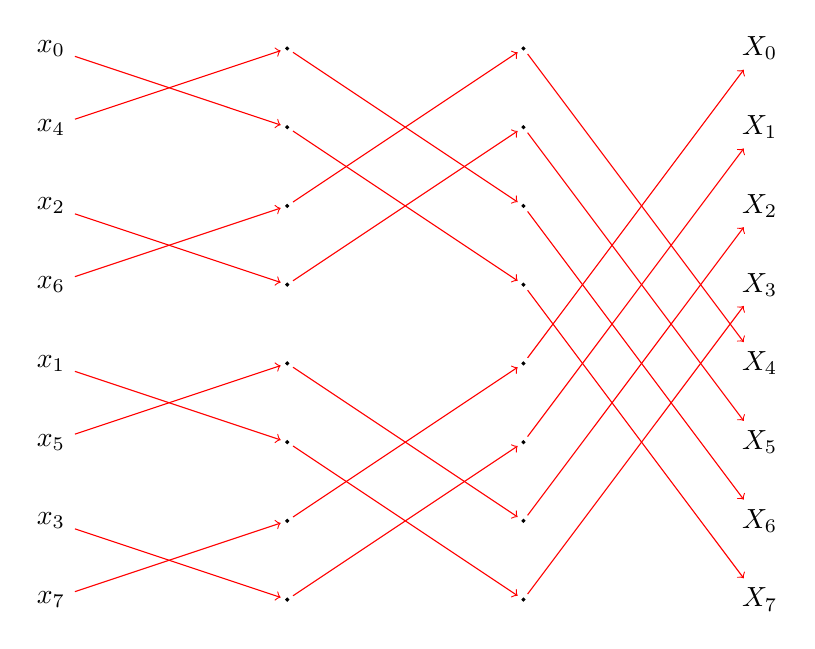
\begin{tikzpicture}[node distance=2cm]

        % nodes
        \node (f0) at (0, 7) {$x_0$};
        \node (f4) at (0, 6) {$x_4$};
        \node (f2) at (0, 5) {$x_2$};
        \node (f6) at (0, 4) {$x_6$};
        \node (f1) at (0, 3) {$x_1$};
        \node (f5) at (0, 2) {$x_5$};
        \node (f3) at (0, 1) {$x_3$};
        \node (f7) at (0, 0) {$x_7$};

        \node [draw,circle,fill=black,inner sep=0pt,outer sep=2pt] (h1) at (3, 7) {};
        \node [draw,circle,fill=black,inner sep=0pt,outer sep=2pt] (h2) at (3, 6) {};
        \node [draw,circle,fill=black,inner sep=0pt,outer sep=2pt] (h3) at (3, 5) {};
        \node [draw,circle,fill=black,inner sep=0pt,outer sep=2pt] (h4) at (3, 4) {};
        \node [draw,circle,fill=black,inner sep=0pt,outer sep=2pt] (h5) at (3, 3) {};
        \node [draw,circle,fill=black,inner sep=0pt,outer sep=2pt] (h6) at (3, 2) {};
        \node [draw,circle,fill=black,inner sep=0pt,outer sep=2pt] (h7) at (3, 1) {};
        \node [draw,circle,fill=black,inner sep=0pt,outer sep=2pt] (h8) at (3, 0) {};

        \node [draw,circle,fill=black,inner sep=0pt,outer sep=2pt] (2h1) at (6, 7) {};
        \node [draw,circle,fill=black,inner sep=0pt,outer sep=2pt] (2h2) at (6, 6) {};
        \node [draw,circle,fill=black,inner sep=0pt,outer sep=2pt] (2h3) at (6, 5) {};
        \node [draw,circle,fill=black,inner sep=0pt,outer sep=2pt] (2h4) at (6, 4) {};
        \node [draw,circle,fill=black,inner sep=0pt,outer sep=2pt] (2h5) at (6, 3) {};
        \node [draw,circle,fill=black,inner sep=0pt,outer sep=2pt] (2h6) at (6, 2) {};
        \node [draw,circle,fill=black,inner sep=0pt,outer sep=2pt] (2h7) at (6, 1) {};
        \node [draw,circle,fill=black,inner sep=0pt,outer sep=2pt] (2h8) at (6, 0) {};

        \node (3h1) at (9, 7) {$X_0$};
        \node (3h2) at (9, 6) {$X_1$};
        \node (3h3) at (9, 5) {$X_2$};
        \node (3h4) at (9, 4) {$X_3$};
        \node (3h5) at (9, 3) {$X_4$};
        \node (3h6) at (9, 2) {$X_5$};
        \node (3h7) at (9, 1) {$X_6$};
        \node (3h8) at (9, 0) {$X_7$};

        % arrows
        % First iteration
        \draw [->,draw=red] (f0) -- (h2);
        \draw [->,draw=red] (f4) -- (h1);
        \draw [->,draw=red] (f2) -- (h4);
        \draw [->,draw=red] (f6) -- (h3);
        \draw [->,draw=red] (f1) -- (h6);
        \draw [->,draw=red] (f5) -- (h5);
        \draw [->,draw=red] (f3) -- (h8);
        \draw [->,draw=red] (f7) -- (h7);

        % Second iteration
        \draw [->,draw=red] (h1) -- (2h3);
        \draw [->,draw=red] (h2) -- (2h4);
        \draw [->,draw=red] (h3) -- (2h1);
        \draw [->,draw=red] (h4) -- (2h2);
        \draw [->,draw=red] (h5) -- (2h7);
        \draw [->,draw=red] (h6) -- (2h8);
        \draw [->,draw=red] (h7) -- (2h5);
        \draw [->,draw=red] (h8) -- (2h6);

        % Third iteration
        \draw [->,draw=red] (2h1) -- (3h5);
        \draw [->,draw=red] (2h2) -- (3h6);
        \draw [->,draw=red] (2h3) -- (3h7);
        \draw [->,draw=red] (2h4) -- (3h8);
        \draw [->,draw=red] (2h5) -- (3h1);
        \draw [->,draw=red] (2h6) -- (3h2);
        \draw [->,draw=red] (2h7) -- (3h3);
        \draw [->,draw=red] (2h8) -- (3h4);
    \end{tikzpicture}
    \caption{Butterfly update for 8 values \cite{fft:derivation}}
    \label{fig:general:butterfly}
\end{figure}
\fi

\ifrelease
\begin{table}
    \centering
    \caption{Bit reversal conversion table for input size 8}
    \label{tab:rev:table}
    \begin{tabular}{|r|r||r|r|}
        \hline
        \textbf{normal dec} & \textbf{normal bin} & \textbf{reversed bin} & \textbf{reversed dec}\\
        \hline
        \texttt{0} & \texttt{000} & \texttt{000} & \texttt{0} \\
        \texttt{1} & \texttt{001} & \texttt{100} & \texttt{4} \\
        \texttt{2} & \texttt{010} & \texttt{010} & \texttt{2} \\
        \texttt{3} & \texttt{011} & \texttt{110} & \texttt{6} \\
        \texttt{4} & \texttt{100} & \texttt{001} & \texttt{1} \\
        \texttt{5} & \texttt{101} & \texttt{101} & \texttt{5} \\
        \texttt{6} & \texttt{110} & \texttt{011} & \texttt{3} \\
        \texttt{7} & \texttt{111} & \texttt{111} & \texttt{7} \\
        \hline
    \end{tabular}
\end{table}
\fi

\ifrelease
\begin{figure}
    \centering
    \begin{tikzpicture}[node distance=2cm]

        % nodes
        \node (A) at (0, 0) {$x_b$};
        \node (B) at (0, 1) {$x_a$};
        \node (C) at (3, 0) {$x'_b$};
        \node (D) at (3, 1) {$x'_a$};

        \node [draw,circle,above left=-3mm and 2mm of D,inner sep=0pt] (plus) {$+$};
        \node [draw,circle,below left=-3mm and 2mm of C,inner sep=0pt] (plus) {$-$};
        \node [draw,circle,below right=-2mm and 2mm of A,inner sep=0pt] (plus) {$\times$};

        % arrows
        \draw [->,draw=red] (A) -- (D);
        \draw [->,draw=red] (B) -- (C);

    \end{tikzpicture}
    \caption{Butterfly update \cite{fft:derivation}}
    \label{fig:butterfly:update}
\end{figure}
\fi

When we have achieved this, the operation order must be established. For the first iteration, the size of the gap between the operands is one. The next gap size is two and the third is four. It is now possible to construct an iterative algorithm. This process is shown in pseudocode in Algorithm~\ref{alg:fft}. The fist part of the algorithm is the Bit reversal. This has clearly $O(N)$ time complexity assuming the time complexity of bit\_reverse is bounded by the number of bits in an integer. For the butterfly updates, the outer while loop will run for $\log{}N$ iterations and the two inner loops will run a total of $\frac{step}{2} \frac{N}{step} = \frac{N}{2}$ times. It is now clear that the time complexity of this algorithm is $O(N\log{}N)$.


\ifrelease
\begin{figure}[H]
    \begin{algorithm}[H]
        \KwData{Complex array $x = x_1, x_2, ..., x_N$ in time domain}
        \KwResult{Complex array $X = X_1, X_2, ..., X_N$ in frequency domain}

        \tcc{Bit reversal}
        \For{$i\gets 0$ \KwTo $N - 1$}{
            $r \gets$ bit\_reverse($i$)\\
            \If{$r > i$}{
                temp $\gets$ $x$[i]\\
                $x$[i] $\gets$ $x$[r]\\
                $x$[r] $\gets$ temp
            }
        }

        \tcc{Butterfly updates}
        $step \gets 2$\\
        \While{$step \leq N$}{
            \For{$k\gets 0$ \KwTo $step/2 - 1$}{
                \For{$p\gets 0$ \KwTo $N/step - 1$}{
                    $curr\gets p * step + k$\\
                    $x$[$curr$] $= x$[$curr$] $+$ $x$[$curr + step/2$]$*\omega^{k}_{step}$\\
                    $x$[$curr + step/2$] $= x$[$curr$] $-$ $x$[$curr + step/2$]$*\omega^{k}_{step}$
                }
            }
            $step \gets 2*step$
        }
        \textbf{return} $x$
        \caption{Iterative FFT}
        \label{alg:fft}
    \end{algorithm}
\end{figure}
\fi

\newpage
\section{Related work}
A study called \emph{FFT benchmark on Android devices: Java versus JNI} \cite{Jr2013} was published in 2013 and investigated how two implementations of \gls{fft} performed on different Android devices. The main point of the study was to compare how a pure Java implementation would perform compared to a library written in C called \gls{fftw}. The FFTW library supports multi-threaded computation and this aspect is also covered in the study. Their benchmark application was run on 35 different devices with different Android versions to get a wide picture of how the algorithms ran on different phones.

\emph{Evaluating Performance of Android Platform Using Native C for Embedded Systems} \cite{Lee2010} explored how \gls{jni} overhead, arithmetic operations, memory access and heap allocation affected an application written in Java and native C. This study was written in 2010 when the Android \gls{ndk} was relatively new. Since then, many patches has been released, improving performance of code written in native C/C++. In this study, Dalvik VM was the virtual machine that executed the Dalvik bytecode. This study found that the \gls{jni} overhead was insignificant and took 0.15 ms to run in their testing environment. Their test results indicated that C was faster than Java in every case. The performance difference was largest in the memory access test and smallest in floating point calculations.

Published in 2016, \emph{Android App Energy Efficiency: The Impact of Language, Runtime, Compiler, and Implementation} \cite{Chen2016} presented a performance comparison between ART and native on Android. The main focus of the report was to find how much more efficient one of them were in terms of energy consumption. Their tests consisted of measuring battery drainage in power as well as execution time of different algorithms. It also compares performance differences between ART and Dalvik. Their conclusion was that native performed much better than code running on the Dalvik VM. However, code compiled by ART improves greatly from Dalvik and performs almost the same as code compiled by Android \gls{ndk}.
